\sloppy
\section{Einleitung}
\label{sec:Einleitung}
In der COVID-19-Pandemie sind Veranstaltungen mit mehreren Teilnehmern mit einem erhöhten Infektionsrisiko verbunden, gerade in geschlossenen Räumen.
Häufig besteht an die Veranstalter eine Pflicht Ein- und Austrittszeitpunkt aller Teilnehmer individuell festzuhalten, um im Falle einer nachträglich auftretenden Infektion die Kontaktverfolgung für die Gesundheitsämter möglichst effizient zu gestalten.
Eine Verwaltung mit Papierformularen ist mit einem hohen Digitalisierungsaufwand verbunden.
Die App Kontaktverfolgung versucht dieses Problem zu lösen.

In der App kann eine Nutzerin oder ein Nutzer die Rolle eines Hosts, also eines Gastgebers oder eines Teilnehmers einnehmen.
 Jeder Nutzer hat ein Profil bestehend aus: Name, E-Mail und Telefonnummer.
Hosts erstellen Räume die an eine reale Adresse gebunden sind. Teilnehmer können dann per NFC-Tag oder einen QR Code in diesen Raum eintreten. Ein und Austrittszeitpunkte werden erfasst und in der Datenbank vermerkt.
Die Ein- und Austrittszeitpunkte der Räume können als PDF exportiert werden.
Nach 14 Tagen werden die Daten aus der Datenbank gelöscht. \todo{doppet steht am ende auch nochmal}
\section{Architektur}\todo{längere namen ? (allgemeiner auf bau der App)}
\label{sec:Architektur}
Im Wesentlichen besteht die Architektur der Applikation aus den in \cref{img:dmodel} dargestellten Komponenten. 
Diese sind verschiedene Activites, RoomLifeCycleService, MQTT-Server eine SQL-Lite Datenbank sowie Preferences.\\
Sämtliche benötigten Informationen über den Nutzer der App werden mittels Preferences erfasst. 
Ohne das vollständige Ausfüllen der Preferences ist in Verwenden der App nicht möglich. 
Um später einen eleganten Zugriff auf die Preferences zu erhalten ist eine \textit{MySelf} Klasse implementiert. 
In den Activitys werden den  verwendeten Widgets ihre Funktionen zugewiesen und bilden somit das Userinterface.
 Möchte sich ein Nutzer registrieren werden dessen Daten über die Activitys aufgenommen und an die interne Datenbank weitergeleitet. 
Diese dient zur Speicherung von Nutzerdaten als auch von Veranstaltungsinformationen. 
Möchte ein Nutzer kann per NFC-Tag oder QR-Code einer Veranstaltung beitreten.
 \todo{wenn ein nutzer einer veranstaltung beitritt geschiet dies per NFC-Tag oder QR-Code}
\todo{NFC-Tag oder NFC-Torken}
Wurde der Room-Tag 
\todo{was ist der raum tag ??wurde vorher nicht erklärt weglassen ??} erkannt, werden mittels MQTT-Service die Nutzerdaten aus der Datenbank  an den Host übermittelt.
 Dieser erhält einen neuen Eintrag in seiner Teilnehmerliste.
Veranstaltungen werden durch den RoomLifeCycleService überwacht. Der RoomLifeCycleService enthält einen Timer welcher den Lebenszyklus eines Events steuert. 
Läuft das Timeout ab, verändert sich der Eventstatuts in „geschlossen“. \todo{vielleicht bissle gröber erklären timer und geschlosen kommen in \cref{sec:RoomLifecycleService}}
Für den Datenaustausch zwischen Host und Teilnehmer kommt der MQTT-Service zum Einsatz. 
Verlässt ein Teilnehmer frühzeitig ein Event, so wird das in der Teilnehmerliste des Hosts vermerkt. Die Exittime wird auch lokal bei Ihm übernommen. 
Schließt der Host den Raum, oder läuft das Timeout des Raumes ab, werden alle Teilnehmer aus dem Event entfernt und die aktuelle Zeit als Austrittszeit eingetragen. \todo{alles schon etwas Funktionalität}
\begin{figure}
	\centering
	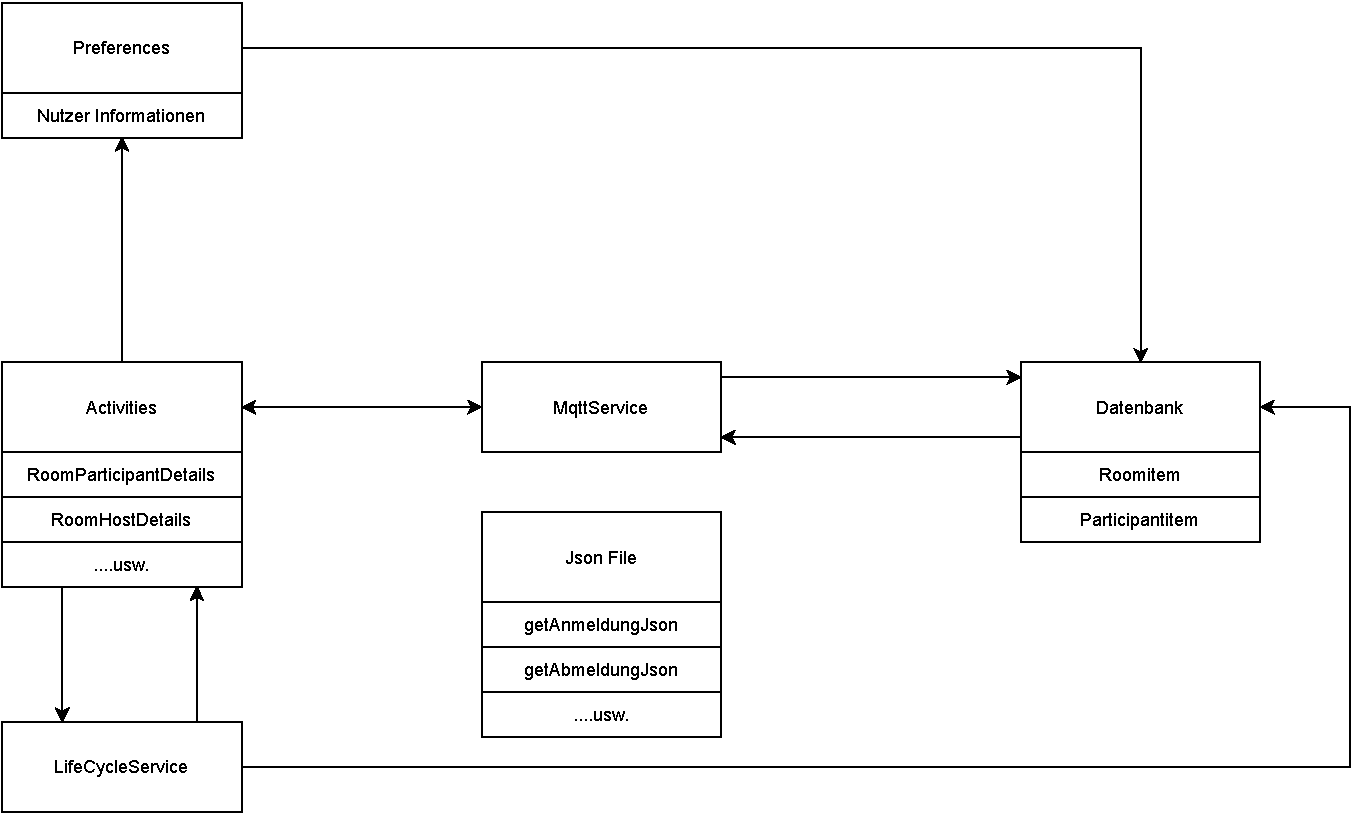
\includegraphics[width =0.9\textwidth]{images/DomaenenModel.pdf}
	\caption{Grundlegendes Domänenmodel der entwickelten App.}
	\label{img:dmodel}
\end{figure}
Die genaueren Funktionsweisen des LifeCycleService, MQTT-Server und SQL-Lite Datenbank werden in den folgenden Kapiteln erläutert.


\section{Datenbank}
\label{sec:Datenbank}
Die Datenbank wird als Speichermedium verwendet, um langfristig Information über Objekte zu halten. 
In der Applikation werden die Tabellenstrukturen durch die Klassen \textit{ParticipantItem} und \textit{RoomItem} umgesetzt. 
\textit{ParticipantItem} ist für die Verwaltung der Nutzerinformationen von Teilnehmern und Host zuständig.\\
 \cref{tab:dbParticipant} zeigt die Struktur der entsprechenden Datenbanktabelle \textit{dbParticipant}.
 Wird die App gestartet müssen in den Preference Angaben über den Namen, Extra, E-Mail und die Telefonnummer eintragen sein, welche dann in einer Participantitem Instanz gekapselt werden. 
\todo{mySelf wird nur in Participant umgewandelt wenn man in ein raum eintritt}
Die Attribute RoomID 
\todo{was genau ist die RaumID(fremdschlüssel auf ein bestimmtes RoomItem in der tabele in welchem sich der Teilnehmer bevindet)} und Entertime erhalten erst beim Betreten einer Veranstaltung einen fixen Wert. Kommt es nun zur Schließung eines Events, können mittels RoomID die dazugehörigen Teilnehmer ermittelt werden. 
Diese erhalten anschließend eine Exittime und werden aus dem Event entfernt. \todo{entfernt werden se ja ned stehn immer noch in der tabelle}\\
Die Tabellenstruktur der Events wird über die \textit{RoomItem} realisiert. Der Aufbau der Tabelle \textit{dbRoom} ist in \cref{tab:dbRoom} dargestellt. 
Beim Erzeugen einer Veranstaltung muss der Eventname, Name des Veranstalters, Ort der Veranstaltung, Zeitraum und Status gespeichert werden. 
Der Status gibt an in welchem aktuellen Zustand sich das Event befindet, hierbei wird zwischen „ROOMWILLOPEN“, „ROOMISOPEN“ oder „ROOMISCLOSE“ unterschieden.
Da Hosts auch die Rolle eines Teilnehmers einnehmen können, wurde hierfür das Feld der FremdID eingeführt. 
Ist das Attribut bei einer Roomitem Instanz initialisiert, wurde dieses Event von einer anderen Person erstellt und man wird als Teilnehmer gelistet.
Weil Datenmanipulationen und Zugriffe nicht im Hauptthread stattfinden dürfen, werden im Repository (Klasse welche Funktionen des Data Access Objects implementiert) alle Datenbankaufrufe in einem Hintergrundthread gestartet.
Die Ausnahme bilden die Funktionen mit der Endung Now. 
Da bei diesen keine Livedata zurückgeben wird dürfen Sie nur für nebenläufige Threads genutzt werden. 
Endet eine Funktion mit dem Suffix Own, werden über diese nur eigens erstellte Veranstaltungen zurückgegeben.
Dies wird vor allem im \textit{RoomLifeCycleService} verwendet damit Teilnehmer nicht, auch wenn es richtig sein sollte, erst bei sich und dann bei den anderen Teilnehmern den Raumstatus z.B. auf ROOMISCLOSE setzen. \todo{komplizierter satz}
 Die Authorität Räume zu öffnen, zu schließen oder das Timeout zu verändern ist allein dem Host vorbehalten.
 Eine genauere Dokumentation der einzelnen Funktionen ist im JavaDoc zu finden.
Da der Lebenszyklus der Activites bei der Verwendung von Datenbanken eine große Rolle  spielt, wird die LiveData-Klasse verwendet, um diesen außer Acht lassen zu können. 

\begin{table}[]
\caption{Struktur der Datenbanktabelle dbParticipant}
\label{tab:dbParticipant}
\centering
\resizebox{0.6\textwidth}{!}{%
\begin{tabular}{l|l|l|l|l|l|l|l}
\toprule
\textbf{id} & \textbf{name}    & \textbf{extra} & \textbf{eMail} & \textbf{phone} & \textbf{roomId} & \textbf{enterTime} & \textbf{exitTime} \\ \midrule
1           & \begin{tabular}[c]{@{}l@{}}Max\\ Mustermann\end{tabular} & null           & mm@mail.de     & 123456789      & 1               & 0                  & 0                 \\ \bottomrule
\end{tabular}%
}
\end{table}


\begin{table}[]
\caption{Struktur der Datenbanktabelle dbRoom}
\label{tab:dbRoom}
\resizebox{\textwidth}{!}{%
\begin{tabular}{l|l|l|l|l|l|l|l|l|l|l|l}
\toprule
\textbf{id} & \textbf{fremdId} & \textbf{roomName} & \textbf{status}                                                                                      & \textbf{host}                                            & \textbf{eMail} & \textbf{phone} & \textbf{place}                                              & \textbf{address} & \textbf{extra} & \textbf{enterTime} & \textbf{exitTime} \\ \midrule
1           & null             & MusterRaum        & 3 (ROOMISCLOSE)  & \begin{tabular}[c]{@{}l@{}}Max\\ Mustermann\end{tabular} & mm@mail.de     & +123456789     & \begin{tabular}[c]{@{}l@{}}12345\\ Musterstadt\end{tabular} & Musterstr. 1     & null           & 0                  & 0                 \\ \bottomrule
\end{tabular}%
}
\end{table}

\section{RoomLifecycleService}\todo{bissle bessere überschrifft ?}
\label{sec:RoomLifecycleService}
Der RoomLifecycleService steuert, wie der Name bereits andeutet, in welchem Zustand sich Räume befinden.
 Der Zustand bestimmt sich maßgeblich nach Öffnungs und Schließzeit.
Diese sind abhängig von der lokalen Zeit. Ein Raum soll ab einer gewissen Uhrzeit geöffnet und zu einer gewissen Uhrzeit geschlossen werden. 
Der LifecycleService gleicht periodisch ab, ob ein Raum gerade geöffnet oder geschlossen sein sollte.
Er wird sowohl im Host, als auch im Teilnehmer-Modus benötigt. 
Die Entscheidung fiel auf einen Service, weil die App auch im nicht-geöffneten Zustand auf Timeouts und Öffnungszeiten reagieren sollte.
Folgender Problemfall: Der Host eröffnet einen Raum und wechselt die App oder sperrt das Smartphone. 
Wenn die Kontaktverfolgungsapp nun nicht mehr im Vordergrund ist während das Timeout ausläuft oder der Raum in die Öffnungszeit reinrutscht, dann würde er nicht geschlossen respektive geöffnet werden. 
Um also zu vermeiden, dass der Host über die gesamte Zeit sein Smartphone nicht verwenden kann und das Display immer angeschaltet bleiben muss, was mit einem hohen Stromverbrauch verbunden ist, fiel die Entscheidung auf einen Service.

Wird der Service gestartet, wird die Raumüberprüfungsroutine nebenläufig in einem neuen Thread gestartet. Das nimmt die Last vom Hauptthread.
Der Raumstatus wird jede Sekunde mit einem Busy-Wait-Algorithmus überprüft.
Das sollte man nicht in den Hauptthread auslagern, da er diesen unnötig blockiert. 
Der Datenbankzugriff ist also nicht die Ursache für die Designentscheidung, denn der Zugriff wird im Repository ohnehin nebenläufig realisiert.
Im Thread wird überprüft ob aktuell geschlossene Räume geöffnet und aktuell geöffnete Räume geschlossen werden sollten.
Nebenher wird im Mainthread versucht den MQTT-Service zu einzubinden. 
Denn der Host soll natürlich auf die MQTT-Topics aller Räume hören die offen sind bzw. aufhören auf alle Räume zu hören die geschlossen sind.
Außerdem muss der Host den Teilnehmern die Raumeigenschaften und den Öffnungsstatus beim Öffnen mitteilen. 
Der MQTT-Service wird hier also gebraucht um den Teilnehmern Raumstatusänderungen mitzuteilen.
Dabei ruft der RoomLifecycleService die Methoden des MQTT-Services nicht direkt auf. Die gesamte Überprüfung der Raumzustände erfolgt nebenläufig in einem anderen Thread. 
Es kann also vorkommen, dass der Thread schon über den MQTT-Service Raumänderungen versendet obwohl er eigentlich noch nicht gebunden ist. 
In dem Fall kommt es zu einer Exception.
Deshalb haben wurde ein Handler eingeführt. Der Thread schreibt in eine threadsichere Liste die Räume rein, die ihren Zustand geändert haben und über MQTT versendet werden sollen. 
Ist der MQTT-Service im Hauptthread gebunden, dann arbeitet besagter Handler mit der Methode \textit{postPendingRooms()} diese Räume im Hauptthread ab. 
Dadurch ist stets sichergestellt, dass der MQTT-Service nur Räume erhält wenn er gebunden ist. 
Dieser Workaround wäre vermeidbar gewesen, wäre Statusüberprüfung und Nachrichtenübertragung in einem zentralen Service realisiert worden. So hätte man gar nicht auf das Binden warten müssen.

Zurück zum LifeCycleService. \todo{bissle andere Formulierung ?}
Ein Raum hat drei mögliche Zustände:
\begin{enumerate}
\item ROOMWILLOPEN
\item ROOMISOPEN
\item ROOMISCLOSE
\end{enumerate}
 Jede Sekunde wird nun überprüft ob Räume die geschlossen sind geöffnet werden sollen, ob Räume die sich öffnen werden geöffnet werden können und ob Räume die geöffnet sind geschlossen werden sollten. 
Falls noch Teilnehmer in zu schließenden Räumen eingebucht sind werden Sie rausgeworfen. In der Datenbank wird dann für alle Teilnehmer als Austrittszeitpunkt die Timeout-Zeit des Raums eingetragen.



\section{MQTT-Service}
\label{sec:MQTT Service}
Der MQTT-Service stellt die MQTT-Funktionalität bereit, über welche die App mit anderen Smartphones kommuniziert.
Das Starten und Stoppen des MQTT-Service findet in der \textit{Activity\_00\_StartActivity} statt. 
Alle anderen Activities binden lediglich den MQTT-Service. Das Binden des MQTT-Service findet in  \textit{Activity\_11\_EnterViaNfcQr}, \textit{Activity\_14\_RoomParticipantsDetails} und \textit{Activity\_22\_RoomHostDetails} statt. 
Des Weiteren wird der Service in dem RoomLivecycle-Service gebunden. 
Näheres hierzu unter \cref{sec:RoomLifecycleService}.  
Beim Verwenden des MQTT-Service wird in jeder Activity geprüft, ob dieser schon gebunden ist (not null). 
Ist dies nicht der Fall, wird das zu sendende Objekt zwischengespeichert und bei erfolgreichem Binden verarbeitet. 
Die im MQTT-Service implementierten Methoden sind ausführlich mittels \href{https://scm.inftech.hs-mannheim.de/gogs/moa/20moagm/src/dev/Doku/javadoc}{JavaDoc} erklärt. 

Die Kommunikation zwischen dem Host und den Teilnehmern verläuft beim MQTT-Protokoll über sogenannte Topics. 
Für einen Raum werden, wie \cref{img:mqtt} zeigt, immer zwei Topics benötigt. 
Der Teilnehmer kann einem Raum über die Topic \textit{moagm/Room-Tag} beitreten. 
Der Host sendet die nötigen Informationen für die Teilnehmer über die Topic \textit{moagm/Room-Tag/public} an alle Teilnehmer. 
Durch die Trennung der Kanäle wird verhindert, dass Teilnehmer die Nachrichten, welche von anderen Teilnehmern an den Host gesendet werden, empfangen können.

Insgesamt gibt es vier verschiedene Nachrichtentypen, welche zwischen den Teilnehmern und dem Host ausgetauscht werden. Alle Nachrichten werden im JSON-Format versendet. 
Dabei lassen sich die Nachrichten in zwei Gruppen unterteilen.
Die Nachrichten \textit{anmeldung.json} und \textit{abmeldung.json} werden vom Teilnehmer an den Host gesendet. 
\textit{teilnehmer.json} und \textit{rauminfo.json} sendet der Host an alle Teilnehmer. 
Mittels eines Converters werden die entsprechenden JSON-Objekte erzeugt und wieder in verwendbare Datentypen zurück gewandelt. 
Zum Identifizieren eines Nachrichtentyps wird (warum auch immer..\todo{Wirklich drin lassen? :)}) nicht das Typfeld benutzt. 
Das Identifizieren wird mit den folgenden Schlüsselworten durchgeführt.
\begin{description}
\item[•] ENTERTIME (\textit{anmeldung.json})
\item[•] EXITTIME (\textit{abmeldung.json})
\item[•] RAUM (\textit{rauminfo.json})
\item[•] TEILNEHMERLIST (\textit{teilnehmer.json})
\end{description}
Abhängig von dem empfangen Datentyp werden unterschiedliche Aktionen durchgeführt.
\\
Mit der in \cref{lst:anmeldung} dargestellten \textit{anmeldung.json} meldet sich ein Teilnehmer beim Host an und stellt eine Verbindung zu der entsprechenden Topic her. In der Nachricht sind alle relevanten Informationen des Teilnehmers enthalten sowie die Uhrzeit wann er den Raum betreten hat.
Informationen über einen Teilnehmer können den Preferences über die \textit{MySelfe} Klasse entnommen werden. 
Der MQTT-Service konvertiert die erhaltene JSON-Nachricht mittels der \textit{AdapterJsonMqtt} Klasse in den passenden Datentyp. 
Das erhalte \textit{ParticipantItem} Objekt wird in der Datenbanktabelle \textit{dbParticipant} mit der  entsprechenden RaumId abgespeichert. 
Die entsprechende RaumId kann der Topic entnommen werden, über welche die JSON-Nachricht empfangen wurde. 
Im Anschluss wird an alle Teilnehmer ein \textit{teilnehmer.json} sowie \textit{rauminfo.json} gesendet.
\begin{figure}
	\centering
	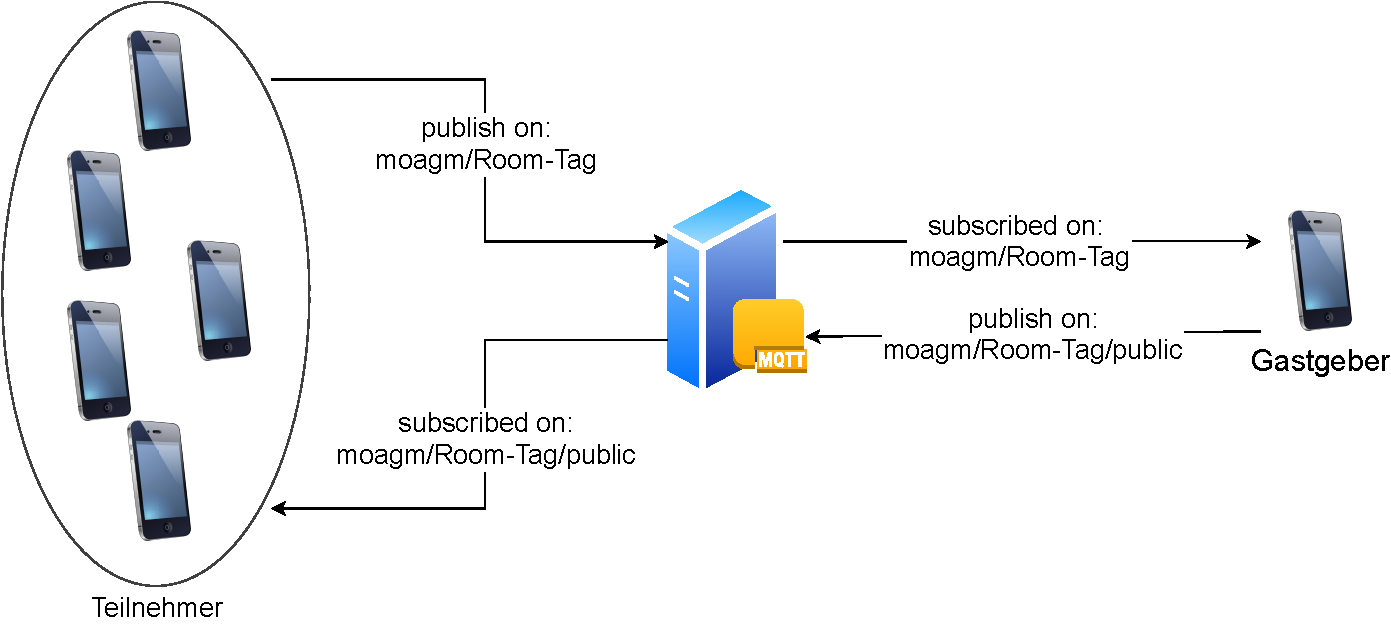
\includegraphics[width =0.9\textwidth]{images/mqttservice.pdf}
	\caption{Darstellung des grundlegenden Kommunikationsablaufes mit MQTT-Topics.}
	\label{img:mqtt}
\end{figure}
\\
Die Nachricht \textit{abmeldung.json}, dargestellt in \cref{lst:abmeldung},   sendet der Teilnehmer an den Host, sobald er den Raum verlässt. 
Dabei meldet sich der Teilnehmer ebenfalls von der entsprechen Topic der MQTT-Verbindung ab. 
Analog zum \textit{anmelden.json} enthält diese Nachricht alle wichtigen Informationen über den Teilnehmer sowie die Uhrzeit zu welcher er den Raum verlässt. 
Im MQTT-Service wird mithilfe des erzeugten \textit{ParticipantItem} Objekt und der RaumId die Exittime des dazugehörenden Teilnehmers aktualisiert.  
\\
\cref{lst:rauminfo} stellt die Nachricht vom Typ \textit{rauminfo.json} da. 
Diese Nachricht enthält sämtliche Informationen über einen Raum. 
Jede vom Teilnehmer empfange \textit{rauminfo.json} wird in ein \textit{RoomItem} Objekt konvertiert und in die Datenbanktabelle \textit{dbRoom} eingefügt bzw. aktualisiert den bereits vorhanden Eintrag. 
Wenn der Host eine \textit{rauminfo.json} versendet, welche den Teilnehmern mitteilt, dass der Raum nun geschlossen ist, meldet der MQTT-Service den Host automatisch von der entsprechenden MQTT-Topic ab.
\\
Der in \cref{lst:teilnehmer} dargestellte Nachrichtentyp \textit{teilnehmer.json} beinhaltet eine Liste aller Teilnehmer eines Raumes. 
Bei Empfangen der Nachricht wird das darin enthaltene JSON-Array in eine Liste von \textit{ParticipantItems} konvertiert. 
Die \textit{ParticipantItems} der Liste werden mit der entsprechenden RaumId, welche über die Topic ermittelbar ist, in die Datenbanktabelle \textit{dbParticipants} eingefügt. 
Um zu verhindern, dass Teilnehmer mehrfach eingetragen werden, wird die Anzahl der bereits eingetragenen Teilnehmer des Raumes ermittelt. 
Aus der Liste der erhaltenen Teilnehmer werden nur \textit{ParticipantItems} eingefügt, welche einen mindestens gleich großen Index besitzen wie die ermittelte Anzahl. 
Diese Variante funktioniert, da sich die Reihenfolge der Teilnehmer in den Datenbanktabellen von Host und Teilnehmer nie ändert.

\begin{minipage}[]{0.45\linewidth}
\begin{lstlisting}[language=json, label={lst:anmeldung}, caption={anmeldung.json}]
{
 "TYPE": "LOGOUT",
 "TEILNEHMER": {
	"NAME": "",
	"EXTRA": "",
	"EMAIL": "",
	"PHONE": ""},
 "EXITTIME": 0
}
\end{lstlisting}
\end{minipage}
\qquad
\begin{minipage}[]{0.45\linewidth}
\begin{lstlisting}[language=json,label={lst:abmeldung}, caption={abmeldung.json}]
{
 "TYPE": "LOGIN",
 "TEILNEHMER": {
	"NAME": "",
	"EXTRA": "",
	"EMAIL": "",
	"PHONE": ""},
 "ENTERTIME": "0"
}
\end{lstlisting}
\end{minipage}
\\
\begin{minipage}[]{0.45\linewidth}
\begin{lstlisting}[language=json, label={lst:rauminfo}, caption={rauminfo.json}]
{
 "TYPE": "RAUMINFO",
 "RAUM": {
	"ID": 0,
	"ROOMNAME": "",
	"STATUS": "",
	"HOST": "",
	"EMAIL": "",
	"PHONE": "",
	"PLACE": "",
	"ADDRESS": "",
	"EXTRA": "",
	"ROOMSTARTTIME": 0,
	"ROOMENDTIME": 0}
}
\end{lstlisting}
\end{minipage}
\qquad
\begin{minipage}[]{0.45\linewidth}
\begin{lstlisting}[language=json, label={lst:teilnehmer}, caption={teilnehmer.json}]
{
 "TYPE": "TEILNEHMER",
 "TEILNEHMERLIST": [
	{
	 "NAME": "",
	 "EXTRA": "",
 	 "EMAIL": "",
 	 "PHONE": "",
 	 "ENTERTIME": 0,
	 "EXITTIME": 0},
	...
 ]
}
\end{lstlisting}
\end{minipage}




\section{Betreten eines Raumes über QR-Code und NFC}
\label{sec:RoomTag - QR und NFC}
Damit Räume distinktiv sind besitzen Sie einen Identifier. Dieser nennt sich Room-Tag und ist zusammengesetzt aus dem Raumnamen, der Email-Adresse des Hosts und der Id des Raums aus der Datenbank des Hosts. 
Beispiel für einen Room-Tags: \textit{Vorlesung 1/dozent@hs-mannheim.de/1}.
Teilnehmer benötigen diesen Tag um dem Raum beizutreten. Dies können Sie über NFC oder über einen QR-Code durchführen. Eine manuelle Eingabe ist nicht implementiert. 

Um den Room-Tag weiterzugeben kann der Veranstalter nach dem Erstellen des Raumes ein PDF generieren und optional per E-Mail versenden. 
Das passiert in der Methode \textit{shareRoom()} in der Klasse \textit{Activity\_22\_RoomHostDetail}. 
In einem solchen PDF ist neben Raum-Metadaten wie Titel, Start und End-Zeitpunkt auch ein QR-Code über den die Teilnehmer beitreten können. 
Für die Erstellung wird die externe Bibliothek zxing von journeyapps benutzt. Die Anbindung erfolgt die Klasse \textit{BarcodeEncoder} in der Klasse \textit{QRCodeManager}. \todo{unvollständiger satz}

Ein Schreiben des Room-Tags auf einen NFC Sticker ist nicht implemenentiert.
 Apps wie \href{https://play.google.com/store/apps/details?id=com.wakdev.wdnfc&hl=de&gl=US}{NFC Tools} des Unternehmens wakdev aus dem PlayStore schaffen hier aber Abhilfe. 
Dort kann der Tag in Plaintext-Format auf den NFC-Tag 
\todo{Tag oder Torken} geschrieben werden.
Eine URI soll nicht vergeben werden, da der Scanner nicht drauf reagiert.
Im Laufe der Entwicklung  wurde fest definiert, dass ein Veranstalter seinen eigenen Raum nicht betreten dürfte.
 Außerdem sollte ein Teilnehmer, nachdem er eine Sitzung verlassen hatte, nicht wieder erneut teilnehmen dürfen. \todo{sollte}
 Damit wurden irreführende Einträge in der Auswertung vermieden. Dieses Verhalten wird mit der Methode \textit{checkEnterPeriomission()} in der \textit{Activity\_11\_EnterViaQrNfc} abgefangen.
\\ 
%\subsubsection*{Betreten eines Raumes über einen QR-Code.}
%\label{paragraph:QR}
Wünscht der Teilnehmer über einen QR-Code einzutreten, dann wird in der \textit{Activity\_11\_EnterViaQrNfc} die Funktion \textit{callScanner()} aus der \textit{QrCodeManager} Klasse gerufen. 
Dort wird die Scanner-Activitiy aus zxing gestartet, die einen Rückgabewert liefert. 
Es ist auch möglich den Scanner zu vorkonfigurieren, so, dass z.B. immer der Kamerablitz angeschaltet ist um auch bei schlechten Licht-Bedingungen den QR-Code gut zu erkennen. 
Außerdem kann ein Timeout eingestellt werden, falls der Nutzer den QR-Code in einer gewissen Zeit nicht einscannt.
In unserem Projekt wurde sich aber wegen der Benutzerfreundlichkeit gegen diese Konfiguration entschieden.
Der Scanner wird über einen Intent gestartet und liefert wenn er fertig ist ein Ergebnis zurück.
Dieses wird in der Methode \textit{onActivityResult()} verarbeitet. Wenn der Scan geklappt hat wird die Methode \textit{enterRoom()} aufgerufen. 
Dort werden die Daten des Room-Tags in die Datenbank eingetragen und die \textit{Activity\_14\_RoomParticipantDetail} gestartet. Der Teilnehmer hört dort dann auf das korrekte MQTT-Topic. Er hat den Raum betreten.\\
%\subsubsection*{Betreten eines Raumes über ein NFC-Torken}
%\label{paragraph:NFC}
Wünscht der Teilnehmer über NFC einzutreten, dann wird in der \textit{Activity\_11\_EnterViaQrNfc} die Funktion \textit{armNFCAdapter()} aufgerufen. Es wird überprüft ob das Smartphone überhaupt einen NFC Sensor hat.
Falls das erfüllt ist wird dieser auf events des Types ACTION\_NDEF\_DISCOVERED scharfgeschaltet. 
Man sagt auch er ist im Foreground-Dispatch-Modus.
Das bedeutet dass, wenn ein neues NFC-Tag detektiert wurde, ein gewisser Intent gestartet wird. 
Falls das der Fall ist, wird die gleiche \textit{Activity\_11\_EnterViaQrNfc} noch einmal gestartet allerdings mit der Action NFC\_INTENT\_ACTION. 
In der \textit{onResume()} wird überprüft ob diese Action gesetzt ist, denn nur dann kehrt die Anwendung aus dem NFC-Intent zurück.
In den Extras des NFC-Intents befindet sich dann er abgelesene Room-Tag. Der Ablauf danach ist wie beim Betreten über einen QR-Code. \textit{enterRoom()} wird gerufen und \textit{Activity\_14\_RoomParticipantDetail} wird gestartet.




\section{PDF}\todo{besserer titel}
\label{sec:PDF}
Das System soll dem Nutzer die Möglichkeit bieten Informationen über einen Raum als PDF zu teilen. 
Dabei gibt es zwei unterschiedliche PDF‘s, diese beinhalten die generellen Rauminformationen, sowie den dazugehörigen QR-Code oder eine Liste aller Teilnehmer.
Das Android-Framework  verfügt über eine \textit{PdfDocument} Klasse, die zum Erstellen von PDF‘s genutzt wird. 
Für eine A4 Seite nach DIN Norm ergeben sich die Werte 846x594 Pixel. Näheres zur Berechnung der Pixelwerte ist unter \href{https://developer.android.com/reference/android/graphics/pdf/PdfDocument.PageInfo}{developer.android} zu finden. D
ie erstellte Seite wird mittels eines Canvas editiert. 
Die Formatierung  der Texte und Grafikelemente lassen sich über die \textit{Paint} Klasse einstellen.
Das erstellte PDF-Dokument wird im externen Dateiverzeichnis der App abgespeichert. Der Nutzer besitzt bei einem fehlgeschlagenen Teilen somit trotzdem die Möglichkeit auf das erstellte PDF zuzugreifen.
Um das PDF zu teilen, wird ein FileProvider verwendet, welcher im Manifest deklariert ist.  Der FileProvider bietet dem Nutzer eine Auswahl der installierten Anwendungen, über welche er das PDF teilen kann.



\section{Sonstiges} \todo{besserer titel}
\label{sec:sonstiges}
Die Anwendung ermöglicht eine effiziente, einfache Möglichkeit dezentral und mit wenig Ressourcen eine Kontaktverfolgung umzusetzen.
Sie erfüllt die Grundsätze der Datenminimierung, Zweckbindung, Richtigkeit und Speicherbegrenzung der Datenschutz Grundverordnung. Nutzerdaten werden nur auf den Endgeräten gespeichert. 
Sie werden nur gespeichert, sollte ein Teilnehmer oder ein Host auch wirklich Kontakt mit diesem Nutzer gehabt haben. 
Außerdem werden alle Einträge die älter als 14 Tage sind aus der Datenbank gelöscht.\\
Die App ist in der Lage bei einem Verlust der Internetverbindung dem Nutzer ein Feedback mitzuteilen und ein hartes Abbrechen zu verhindern. 
Dafür wird ein BroadcastReciever verwendet welcher Auf Netzwerkänderungen hört. 
Der BroadcastReciver wird beim Erstellen des RoomLivecyclesServices an diesen gebunden.
 Bricht die Internetverbindung ab werden alle Services gestoppt. 
Des Weiteren wird dem Nutzer mitgeteilt das die Internetverbindung verloren wurde und er die App mit Internetverbindung neustarten muss.

\section{Fazit und Ausblick}
\label{sec:FuA}

In der Entwicklung konnten die in der Vorlesung gelehrten Inhalte nocheinmal selbstständig angewandt werden. 
Auch verschiedene Nutzungsweisen des Versionsverwaltungstools Git konnten getestet werden. 
Wo am Anfang hauptsächlich auf einem Branch enwickelt wurde, wurde später wurde auf ein Feature-Based-Setup gewechselt in dem jeder Entwickler einen eigenen Branch pro Freature hatte.
Zum Schluss wurde sich für einen dev-branch für experimentelle Änderungen und einen master-branch für stabile Versionen entschieden, da dies gerade für die Demos sehr von Vorteil war. \todo{hinzufügen ob die gestellten ziele erreicht wurden oder nicht}

Für eine Weiterentwicklung der App sind essenzielle Verbesserungen vorzunehmen. Die Services MQTT-Service und RoomLivecycleService müssen in einem einzigen Service zusammengefasst werden. 
Dadurch lässt sich die Fehlerrate welche beim Binden des MQTT-Services entstehen deutlich reduzieren. Auf etwaige Handler könnte verzichtet werden. 
Das Zusammenfassen verringert zudem deutlich die Gesamtkomplexität des Projektes.
 Ebenso muss in der \textit{PdfClass} das PDF mit der Übersicht aller Teilnehmer überarbeitet werden. 
 In der aktuellen Version wird die E-Mail Adresse ab einer bestimmten Länge zum Teil mit in die nächste Spalte geschrieben.
 Ziel ist es, dass in dieser Situation ein automatischer Zeilenumbruch in der entsprechenden Spalte eingefügt wird.
Neben den essenziellen Verbesserungen  wäre eine Implementierung von folgenden Features erwägenswert.
\begin{description}
\item[•]Beschreiben von NFC-Torkens in der App ohne Drittanbieter-App 
\item[•]Profilbild in den Nutzerinformationen
\item[•]Benachrichtigen aller Teilnehmer bei positivem Corona-Befund
\item[•]Eigens URI-Format für NFC Tags
\item[•]Manuelle Eingabe als Möglichkeit einen Raum zu betreten.
\item[•]Chat zwischen Teilnehmern eines Raumes
\item[•]Unittests unter Verwendung der \textit{TestClass} implementieren
\end{description}


Eine verbesserte Version der Kontaktverfolgung App lässt sich ideal in der Hochschule einsetzen. ...\todo{1-2 sätze warum}